%%%%%%%%%%%%%%%%%%%%%%%%%%%%%%%%%%%%%%%%%%%%%%%%%%%%%%%%%%%%%%%%%%%%%%%%%%%%%%%%
%                                                                              %
%            A Painless Introduction to Programming UAMMD Modules              %
%                           Chapter 3: Measuring                               %                                                                              
%                                                                              %
%                          Marc Meléndez Schofield                             %
%                                                                              %
%%%%%%%%%%%%%%%%%%%%%%%%%%%%%%%%%%%%%%%%%%%%%%%%%%%%%%%%%%%%%%%%%%%%%%%%%%%%%%%%

The first two chapters have given you more than enough material to create your 
own simulations and use the output to make videos of spheres flying around and 
colliding in your own virtual world. But scientists aim at describing the real 
world, and that involves measuring interesting quantities in your system and 
relating them to material objects.

\section{Energy and linear momentum}

Physical simulations commonly measure energy. Unexpected fluctuations or drifts 
in the energy often warn us of something askew in our code. Take our bouncing 
rubber ball from the introduction. Its mechanical energy,
\begin{equation*}
  E = \frac{1}{2} m \|\mathbf{v}\|^2 + m|g|y,
\end{equation*}
should remain constant while it flies freely. The absolute value $|g|$ appears 
here instead of plain $g$ because, if you remember, we defined the acceleration 
of gravity as $g = -9.8\ \mathrm{m/s}^2$ in our code. On impact, the ball 
reduced its speed slightly, so we expect a sudden drop in $E$ every time 
the ball hits the floor. As it bounces time and again, leaking more and more 
energy, $E$ will tend towards zero.

Due to numerical rounding in the operations, we shouldn't expect a perfect 
conservation of energy but we obviously want to keep energy fluctuations low, 
below one percent, say. If you have managed to code the algorithm correctly, you 
can usually decrease energy fluctuations further by choosing smaller time steps.

Let's verify our predictions about the bouncing ball program by changing the 
output section. We'll set the mass to $100$ grams.
\begin{lstlisting}
%! codeblock: rubberBallEOutput
    if(printEverynSteps > 0
       && step % printEverynSteps == 0) {

      float m = 0.1; /* Mass */

      /* Mechanical energy */
      float E = 0.5*m*(v[0]*v[0] + v[1]*v[1]) - m*g*r[1];

      cout<<step*dt<<" "<<r[0]<<" "<<r[1]<<" "<<E<<endl;
    } //!
%! codeblockend !//
\end{lstlisting}
Note that I wrote \texttt{-m*g*r[1]} instead of \texttt{+m*g*r[1]} due to the 
negative value of \texttt{g}. Figure \ref{rubberBallE} plots the result, which 
agrees with our predictions precisely.

\begin{figure}
  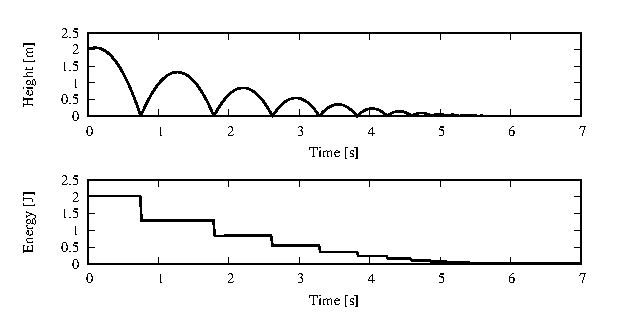
\includegraphics[width = \textwidth]{figures/rubberBallE.eps}
  \caption{\label{rubberBallE}Height (\textit{top}) and mechanical energy 
           (\textit{bottom}) of a one-hundred-gram bouncing ball versus time. 
           The energy remains constant with the ball in free flight, but a 
           fraction is lost when the ball hits the ground.}
\end{figure}

\begin{comment}
rubberBallE.cpp differs only from rubberBall.cpp in the code snippet mentioned 
above.
%! codefile: code/rubberBallE.cpp
# include <iostream>

using std::cout;
using std::endl;

int main(int argc, char * argv[])
{
  /* State of the rubber ball */
  float r[2]; /* Position (measured in metres) */
  float v[2]; /* Velocity (in metres/second) */

  float g = -9.8; /* Acceleration of gravity (in m/s^2) */

  /* Integration parameters */
  int nsteps = 10000; /* Number of time steps to calculate */
  float dt = 0.001; /* Size of time step (in seconds) */
  int printEverynSteps = 20;

  /* Initial conditions */
  r[0] = 0;
  r[1] = 2;
  v[0] = 0.5;
  v[1] = 1;

  /* Euler integration of the equations of motion */
  for(int step = 0; step <= nsteps; ++step) {
    /* New position */
    r[0] = r[0] + v[0]*dt;
    r[1] = r[1] + v[1]*dt;

    /* New velocity */
    v[1] = v[1] + g*dt;

    /* Deal with collisions */
    if(r[1] <= 0 && v[1] < 0) {
      v[0] = 0.9*v[0];
      v[1] = -0.8*v[1];
    }

    /* Output state */
    %! codeinsert: rubberBallEOutput
  }
  cout<<"# Simulated time: "<<nsteps*dt<<" seconds. #"<<endl;
  return 0;
}
%! codeend
\end{comment}

Returning to UAMMD, let's write a function that outputs the total energy of the 
system. Each interactor has a \texttt{sumEnergy} method that calculates the 
potential energy due to corresponding interaction for each particle and adds it 
to the energy vector that we access with \texttt{getEnergy}. You can add the 
kinetic energy by calling the interactor's \texttt{sumEnergy}.

To begin with, our new \texttt{getTotalEnergy} function will clear the energy 
vector and initialize the \texttt{totalEnergy} variable to zero.
\begin{lstlisting}
%! codeblock: getTotalEnergy
double getTotalEnergy(std::shared_ptr<Integrator> integrator,
                      std::shared_ptr<ParticleData> particles){
  {
    auto energy
      = particles->getEnergy(access::location::cpu,
                             access::mode::write);
    std::fill(energy.begin(), energy.end(), real(0.0));
  }

  double totalEnergy = 0; //!
  %! codeinsert: getKineticEnergy
  %! codeinsert: getPotentialEnergy
  %! codeinsert: reduceEnergyVector
%! codeblockend !//
\end{lstlisting}
Next, it sums the kinetic energies to the particle energy vector.
\begin{lstlisting}
%! codeblock: getKineticEnergy
  integrator->sumEnergy(); //!
%! codeblockend !//
\end{lstlisting}
After that, it adds in the potential energies from interactions.
\begin{lstlisting}
%! codeblock: getPotentialEnergy
  for(auto interactor: integrator->getInteractors()){
    interactor->sumEnergy();
  } //!
%! codeblockend !//
\end{lstlisting}
Finally, we add all the values in the energy vector and return the grand total.
\begin{lstlisting}
%! codeblock: reduceEnergyVector
  {
    auto energy
      = particles->getEnergy(access::location::cpu,
                             access::mode::read);
    for(int i = 0; i < particles->getNumParticles(); ++i) {
      totalEnergy += energy[i];
    }
  }
  return totalEnergy;
} //!
%! codeblockend !//
\end{lstlisting}

Similarly, we can write a function to calculate the total linear momentum 
vector, which should remain approximately constant in the absence of external 
force fields.

\begin{lstlisting}
%! codeblock: getTotalMomentum
real3 getTotalMomentum(std::shared_ptr<ParticleData> particles){
    auto velocity
      = particles->getVel(access::location::cpu,
                          access::mode::read);
    auto mass
      = particles->getMass(access::location::cpu,
                           access::mode::read);

    real3 totalMomentum = make_real3(0.0, 0.0, 0.0);

    for(int i = 0; i < particles->getNumParticles(); ++i) {
      totalMomentum += mass[i]*velocity[i];
    }

  return totalMomentum;
} //!
%! codeblockend !//
\end{lstlisting}

\section{Temperature}

The Verlet (NVE) algorithm should conserve energy and linear momentum, so we 
often rely on these quantities to signal mistakes in our code. Precisely because 
they remain constant, they do not give us much interesting information when the 
simulation runs smoothly. The values coincide approximately with those of the 
initial state we set up.

The temperature connects the microscopic world of molecular collisions with the 
macroscopic world of flasks and thermometers. The equipartition theorem states 
that the expected value of a particle at equilibrium equals
\begin{equation*}
  \frac{1}{2} m \left\langle v^2 \right\rangle = \frac{3}{2}k_B T,
\end{equation*}
where $k_B$ stands for Boltzmann's constant and $T$ for the absolute 
temperature. The term on the left refers to the average kinetic energy with 
respect to the centre of mass of the system.

The equation above provides a convenient way of determining the temperature of a 
system once it equilibrates. Instead of $T$, we will write a function to 
calculate $k_BT$ and refer to this magnitude as the \textit{thermal energy}.

We start by calculating the velocity of the centre of mass, \texttt{Vcm}, and 
the total mass, \texttt{M}.
\begin{lstlisting}
%! codeblock: getThermalEnergy
double getThermalEnergy(std::shared_ptr<ParticleData> particles){
  int N = particles->getNumParticles();
  auto velocity
    = particles->getVel(access::location::cpu,
                          access::mode::read);
  auto mass
    = particles->getMass(access::location::cpu,
                           access::mode::read);

  real3 Vcm = make_real3(0.0, 0.0, 0.0);
  double M = real(0.0);

  for(int i = 0; i < N; ++i) {
    Vcm += mass[i]*velocity[i];
    M += mass[i];
  }
  Vcm /= M; //!
  %! codeinsert: getThermalKinetic
%! codeblockend !//
\end{lstlisting}
Then we calculate the total kinetic energy with respect to the centre of mass 
and return two thirds of the average kinetic energy per particle.
\begin{lstlisting}
%! codeblock: getThermalKinetic
  double kineticEnergy = real(0.0);
  for(int i = 0; i < N; ++i) {
    kineticEnergy
     += real(0.5)*mass[i]*dot(velocity[i] - Vcm, velocity[i] - Vcm);
  }

  return real(2.0/(3.0*N))*kineticEnergy;
}//!
%! codeblockend !//
\end{lstlisting}

% Simulation results

% Heat capacity

\begin{comment}
\begin{lstlisting}
%! codefile: code/measurements.cu
# include "uammd.cuh"
# include "utils/InputFile.h"
# include "utils/InitialConditions.cuh"
# include "Interactor/Potential/Potential.cuh"
# include "Interactor/NeighbourList/CellList.cuh"
# include "Interactor/PairForces.cuh"
# include "Integrator/VerletNVE.cuh"

using namespace uammd;
using std::make_shared;
using std::endl;

struct InputParameters {
  int numberOfParticles;
  real L;
  real dt;
  real epsilon;
  real sigma;
  real mass;
  real cutOff;
  real particleEnergy;
  std::string outputFile;
  std::string macroFile;
  int numberOfSteps;
  int printEverynSteps;
};

InputParameters readParameterFile(std::shared_ptr<System> sys)
{
  if(!std::ifstream("data.main").good()) {
    sys->log<System::WARNING>("File data.main not found. Creating file with default values.");
    std::ofstream defaultParameters("data.main");
    if(not defaultParameters.is_open()) {
      sys->log<System::CRITICAL>("Unable to create data.main file. Halting program.");
      exit(-1);
    }
    defaultParameters<<"numberOfParticles 100000"<<endl;
    defaultParameters<<"boxSize 128"<<endl;
    defaultParameters<<"timeStep 0.01"<<endl;
    defaultParameters<<"epsilon 1.0"<<endl;
    defaultParameters<<"sigma 1.0"<<endl;
    defaultParameters<<"mass 1.0"<<endl;
    defaultParameters<<"cutOff 2.5"<<endl;
    defaultParameters<<"particleEnergy 1.0"<<endl;
    defaultParameters<<"outputFile Lennard-Jones.dat"<<endl;
    defaultParameters<<"measurementsFile LJmacro.dat"<<endl;
    defaultParameters<<"numberOfSteps 10000"<<endl;
    defaultParameters<<"printEverynSteps 1000"<<endl;
  }
  InputFile parameterFile("data.main", sys);
  InputParameters params;

  parameterFile.getOption("numberOfParticles",
    InputFile::Required)>>params.numberOfParticles;
  parameterFile.getOption("boxSize",
    InputFile::Required)>>params.L;
  parameterFile.getOption("timeStep",
    InputFile::Required)>>params.dt;
  parameterFile.getOption("epsilon",
    InputFile::Required)>>params.epsilon;
  parameterFile.getOption("sigma",
    InputFile::Required)>>params.sigma;
  parameterFile.getOption("mass",
    InputFile::Required)>>params.mass;
  parameterFile.getOption("cutOff",
    InputFile::Required)>>params.cutOff;
  parameterFile.getOption("particleEnergy",
    InputFile::Required)>>params.particleEnergy;
  parameterFile.getOption("outputFile",
    InputFile::Required)>>params.outputFile;
  parameterFile.getOption("measurementsFile",
    InputFile::Required)>>params.macroFile;
  parameterFile.getOption("numberOfSteps",
    InputFile::Required)>>params.numberOfSteps;
  parameterFile.getOption("printEverynSteps",
    InputFile::Required)>>params.printEverynSteps;

  return params;
}

%! codeinsert: getTotalEnergy

%! codeinsert: getTotalMomentum

%! codeinsert: getThermalEnergy

int main(int argc, char *argv[]){

  auto sys = make_shared<System>(argc, argv);

  %! codeinsert: loadParameters src: chapters/first_simulation.tex

  int numberOfParticles = simParams.numberOfParticles;
  auto particles
    = make_shared<ParticleData>(numberOfParticles, sys);

  real L = simParams.L;

  %! codeinsert: LJsimulationBox src: chapters/first_simulation.tex
  {
    auto position
      = particles->getPos(access::location::cpu,
                          access::mode::write);

    auto initial =  initLattice(box.boxSize,
                                numberOfParticles, sc);

    std::copy(initial.begin(), initial.end(), position.begin());
  }
  {
    auto mass
      = particles->getMass(access::location::cpu,
                           access::mode::write);
    std::fill(mass.begin(), mass.end(), simParams.mass);
  }

  using Verlet = VerletNVE;
  Verlet::Parameters VerletParams;
  VerletParams.dt = simParams.dt;
  VerletParams.initVelocities = true;
  VerletParams.energy = simParams.particleEnergy;

  %! codeinsert: Verlet src: chapters/first_simulation.tex

  auto LJPotential = make_shared<Potential::LJ>(sys);
  {
    Potential::LJ::InputPairParameters LJParams;
    LJParams.epsilon = simParams.epsilon;
    LJParams.sigma = simParams.sigma;
    LJParams.cutOff = simParams.cutOff;
    LJParams.shift = true;
    LJPotential->setPotParameters(0, 0, LJParams);
  }

  %! codeinsert: Lennard-JonesInteraction src: chapters/first_simulation.tex

  std::string outputFile = simParams.outputFile;
  std::ofstream out(outputFile);

  std::string macroFile = simParams.macroFile;
  std::ofstream macro(macroFile);

  int numberOfSteps = simParams.numberOfSteps;
  int printEverynSteps = simParams.printEverynSteps;

  for(int step = 0; step < numberOfSteps; ++step) {
    integrator->forwardTime();

    if(printEverynSteps > 0
       and step % printEverynSteps == 1) {

      auto position
        = particles->getPos(access::location::cpu,
                            access::mode::read);
      const int * index = particles->getIdOrderedIndices(access::location::cpu);

      out<<endl;
      for(int id = 0; id < numberOfParticles; ++id)
        out<<box.apply_pbc(make_real3(position[index[id]]))<<endl; //!

      macro<<step*simParams.dt<<" ";
      macro<<getTotalEnergy(integrator, particles)<<" ";
      macro<<getTotalMomentum(particles)<<" ";
      macro<<getThermalEnergy(particles)<<endl;
    }
  }

  sys->finish();

  return 0;
}
%! codeend
\end{lstlisting}
\end{comment}


\section{Thermostats}

Langevin thermostat

Brownian Dynamics

MSD

\section{Structure}

Histograms

RDF

\section{Pressure}

RDF

Virial

Barostats

\section{Check points}

\begin{comment}
List of programs written in this chapter:
%! codeblock: codelist
* `rubberBallE.cpp`: A version of the `rubberBall.cpp` from the introduction 
   which also outputs the mechanical energy of the ball.
* `measurements.cu`:
%! codeblockend
\end{comment}
